% Options for packages loaded elsewhere
\PassOptionsToPackage{unicode}{hyperref}
\PassOptionsToPackage{hyphens}{url}
%
\documentclass[
  12pt,
]{article}
\usepackage{lmodern}
\usepackage{amssymb,amsmath}
\usepackage{ifxetex,ifluatex}
\ifnum 0\ifxetex 1\fi\ifluatex 1\fi=0 % if pdftex
  \usepackage[T1]{fontenc}
  \usepackage[utf8]{inputenc}
  \usepackage{textcomp} % provide euro and other symbols
\else % if luatex or xetex
  \usepackage{unicode-math}
  \defaultfontfeatures{Scale=MatchLowercase}
  \defaultfontfeatures[\rmfamily]{Ligatures=TeX,Scale=1}
\fi
% Use upquote if available, for straight quotes in verbatim environments
\IfFileExists{upquote.sty}{\usepackage{upquote}}{}
\IfFileExists{microtype.sty}{% use microtype if available
  \usepackage[]{microtype}
  \UseMicrotypeSet[protrusion]{basicmath} % disable protrusion for tt fonts
}{}
\makeatletter
\@ifundefined{KOMAClassName}{% if non-KOMA class
  \IfFileExists{parskip.sty}{%
    \usepackage{parskip}
  }{% else
    \setlength{\parindent}{0pt}
    \setlength{\parskip}{6pt plus 2pt minus 1pt}}
}{% if KOMA class
  \KOMAoptions{parskip=half}}
\makeatother
\usepackage{xcolor}
\IfFileExists{xurl.sty}{\usepackage{xurl}}{} % add URL line breaks if available
\IfFileExists{bookmark.sty}{\usepackage{bookmark}}{\usepackage{hyperref}}
\hypersetup{
  pdftitle={Exercise 3 Solutions},
  pdfauthor={Ian McCarthy, Econ 771},
  hidelinks,
  pdfcreator={LaTeX via pandoc}}
\urlstyle{same} % disable monospaced font for URLs
\usepackage[left=2cm,right=2cm,top=1cm,bottom=2cm]{geometry}
\usepackage{color}
\usepackage{fancyvrb}
\newcommand{\VerbBar}{|}
\newcommand{\VERB}{\Verb[commandchars=\\\{\}]}
\DefineVerbatimEnvironment{Highlighting}{Verbatim}{commandchars=\\\{\}}
% Add ',fontsize=\small' for more characters per line
\usepackage{framed}
\definecolor{shadecolor}{RGB}{248,248,248}
\newenvironment{Shaded}{\begin{snugshade}}{\end{snugshade}}
\newcommand{\AlertTok}[1]{\textcolor[rgb]{0.94,0.16,0.16}{#1}}
\newcommand{\AnnotationTok}[1]{\textcolor[rgb]{0.56,0.35,0.01}{\textbf{\textit{#1}}}}
\newcommand{\AttributeTok}[1]{\textcolor[rgb]{0.77,0.63,0.00}{#1}}
\newcommand{\BaseNTok}[1]{\textcolor[rgb]{0.00,0.00,0.81}{#1}}
\newcommand{\BuiltInTok}[1]{#1}
\newcommand{\CharTok}[1]{\textcolor[rgb]{0.31,0.60,0.02}{#1}}
\newcommand{\CommentTok}[1]{\textcolor[rgb]{0.56,0.35,0.01}{\textit{#1}}}
\newcommand{\CommentVarTok}[1]{\textcolor[rgb]{0.56,0.35,0.01}{\textbf{\textit{#1}}}}
\newcommand{\ConstantTok}[1]{\textcolor[rgb]{0.00,0.00,0.00}{#1}}
\newcommand{\ControlFlowTok}[1]{\textcolor[rgb]{0.13,0.29,0.53}{\textbf{#1}}}
\newcommand{\DataTypeTok}[1]{\textcolor[rgb]{0.13,0.29,0.53}{#1}}
\newcommand{\DecValTok}[1]{\textcolor[rgb]{0.00,0.00,0.81}{#1}}
\newcommand{\DocumentationTok}[1]{\textcolor[rgb]{0.56,0.35,0.01}{\textbf{\textit{#1}}}}
\newcommand{\ErrorTok}[1]{\textcolor[rgb]{0.64,0.00,0.00}{\textbf{#1}}}
\newcommand{\ExtensionTok}[1]{#1}
\newcommand{\FloatTok}[1]{\textcolor[rgb]{0.00,0.00,0.81}{#1}}
\newcommand{\FunctionTok}[1]{\textcolor[rgb]{0.00,0.00,0.00}{#1}}
\newcommand{\ImportTok}[1]{#1}
\newcommand{\InformationTok}[1]{\textcolor[rgb]{0.56,0.35,0.01}{\textbf{\textit{#1}}}}
\newcommand{\KeywordTok}[1]{\textcolor[rgb]{0.13,0.29,0.53}{\textbf{#1}}}
\newcommand{\NormalTok}[1]{#1}
\newcommand{\OperatorTok}[1]{\textcolor[rgb]{0.81,0.36,0.00}{\textbf{#1}}}
\newcommand{\OtherTok}[1]{\textcolor[rgb]{0.56,0.35,0.01}{#1}}
\newcommand{\PreprocessorTok}[1]{\textcolor[rgb]{0.56,0.35,0.01}{\textit{#1}}}
\newcommand{\RegionMarkerTok}[1]{#1}
\newcommand{\SpecialCharTok}[1]{\textcolor[rgb]{0.00,0.00,0.00}{#1}}
\newcommand{\SpecialStringTok}[1]{\textcolor[rgb]{0.31,0.60,0.02}{#1}}
\newcommand{\StringTok}[1]{\textcolor[rgb]{0.31,0.60,0.02}{#1}}
\newcommand{\VariableTok}[1]{\textcolor[rgb]{0.00,0.00,0.00}{#1}}
\newcommand{\VerbatimStringTok}[1]{\textcolor[rgb]{0.31,0.60,0.02}{#1}}
\newcommand{\WarningTok}[1]{\textcolor[rgb]{0.56,0.35,0.01}{\textbf{\textit{#1}}}}
\usepackage{longtable,booktabs}
% Correct order of tables after \paragraph or \subparagraph
\usepackage{etoolbox}
\makeatletter
\patchcmd\longtable{\par}{\if@noskipsec\mbox{}\fi\par}{}{}
\makeatother
% Allow footnotes in longtable head/foot
\IfFileExists{footnotehyper.sty}{\usepackage{footnotehyper}}{\usepackage{footnote}}
\makesavenoteenv{longtable}
\usepackage{graphicx}
\makeatletter
\def\maxwidth{\ifdim\Gin@nat@width>\linewidth\linewidth\else\Gin@nat@width\fi}
\def\maxheight{\ifdim\Gin@nat@height>\textheight\textheight\else\Gin@nat@height\fi}
\makeatother
% Scale images if necessary, so that they will not overflow the page
% margins by default, and it is still possible to overwrite the defaults
% using explicit options in \includegraphics[width, height, ...]{}
\setkeys{Gin}{width=\maxwidth,height=\maxheight,keepaspectratio}
% Set default figure placement to htbp
\makeatletter
\def\fps@figure{htbp}
\makeatother
\setlength{\emergencystretch}{3em} % prevent overfull lines
\providecommand{\tightlist}{%
  \setlength{\itemsep}{0pt}\setlength{\parskip}{0pt}}
\setcounter{secnumdepth}{-\maxdimen} % remove section numbering
\usepackage{setspace}
\usepackage{titlesec}
\titlespacing{\title}{0pt}{\parskip}{-\parskip}
\titlespacing{\section}{0pt}{12pt plus 2pt minus 1pt}{0pt plus 1pt minus 1pt}
\titlespacing{\subsection}{0pt}{12pt plus 2pt minus 1pt}{0pt plus 1pt minus 1pt}
\titlespacing{\subsubsection}{0pt}{12pt plus 2pt minus 1pt}{0pt plus 1pt minus 1pt}
\usepackage{float}
\usepackage{booktabs}
\usepackage{longtable}
\usepackage{array}
\usepackage{multirow}
\usepackage{wrapfig}
\usepackage{float}
\usepackage{colortbl}
\usepackage{pdflscape}
\usepackage{tabu}
\usepackage{threeparttable}
\usepackage{threeparttablex}
\usepackage[normalem]{ulem}
\usepackage{makecell}
\usepackage{xcolor}
\newlength{\cslhangindent}
\setlength{\cslhangindent}{1.5em}
\newenvironment{cslreferences}%
  {\setlength{\parindent}{0pt}%
  \everypar{\setlength{\hangindent}{\cslhangindent}}\ignorespaces}%
  {\par}

\title{Exercise 3 Solutions}
\author{Ian McCarthy, Econ 771}
\date{Fall 2020}

\begin{document}
\maketitle

\setstretch{1.5}

\hypertarget{overview}{%
\section{Overview}\label{overview}}

This document lays out my approach to addressing the questions in Exercise 3. There are lots of ways to answer these problems and build the data, especially in \texttt{R}! My way of answering the questions is just one of many.

I also have a particular workflow that you may or may not choose to adopt. That workflow is to do all of my analysis seperately from my markdown document. I really don't like seeing huge markdown documents constantly going in and out of data work and discussion. It's also not feasible to work with really large data within the markdown document. So, I do all of the analysis, remove any large objects (including the data), keep only the relevant objects for the final markdown (figures, tables, specific numbers or statistics), and then save the workspace. Then I load the workspace into my markdown document.

\hypertarget{data}{%
\section{Data}\label{data}}

The data in this assignment are straightforward since we're working directly off of Ericson (2014). All of the data are available on the journal website for the paper, \href{https://www.aeaweb.org/articles?id=10.1257/pol.6.1.38}{here}.

Still, it might take some time to understand the data and variable construction. The data are organized into two datasets: 1) the prescription drug plan data in the \texttt{Data\_main.dta} file; and 2) the subsidy information in the \texttt{Data\_subsidyinfo.dta} file. Before merging these data, I first create the market share variable in the PDP data as follows:

\setstretch{1}

\begin{Shaded}
\begin{Highlighting}[]
\NormalTok{pdp.data \textless{}{-}}\StringTok{ }\NormalTok{pdp.data }\OperatorTok{\%\textgreater{}\%}
\StringTok{  }\KeywordTok{group\_by}\NormalTok{(state, year) }\OperatorTok{\%\textgreater{}\%}
\StringTok{  }\KeywordTok{mutate}\NormalTok{(}\DataTypeTok{state\_yr\_enroll =} \KeywordTok{sum}\NormalTok{(enrollment, }\DataTypeTok{na.rm=}\OtherTok{TRUE}\NormalTok{)) }\OperatorTok{\%\textgreater{}\%}
\StringTok{  }\KeywordTok{ungroup}\NormalTok{() }\OperatorTok{\%\textgreater{}\%}
\StringTok{  }\KeywordTok{mutate}\NormalTok{(}\DataTypeTok{share =}\NormalTok{ enrollment}\OperatorTok{/}\NormalTok{state\_yr\_enroll,}
         \DataTypeTok{ln\_share =} \KeywordTok{log}\NormalTok{(share))}
\end{Highlighting}
\end{Shaded}

\setstretch{1.5}

Then I reshape (or \texttt{pivot\_longer} in \texttt{R}) the subsidy data so that it matches the format of the PDP data.

\setstretch{1}

\begin{Shaded}
\begin{Highlighting}[]
\NormalTok{lis.data \textless{}{-}}\StringTok{ }\KeywordTok{pivot\_longer}\NormalTok{(lis.data, }\DataTypeTok{cols=}\KeywordTok{c}\NormalTok{(}\StringTok{"s2006"}\NormalTok{,}\StringTok{"s2007"}\NormalTok{,}\StringTok{"s2008"}\NormalTok{,}\StringTok{"s2009"}\NormalTok{,}\StringTok{"s2010"}\NormalTok{), }
                         \DataTypeTok{names\_to=}\StringTok{"year"}\NormalTok{,}
                         \DataTypeTok{names\_prefix=}\StringTok{"s"}\NormalTok{,}
                         \DataTypeTok{values\_to=}\StringTok{"LISsubsidy"}\NormalTok{) }\OperatorTok{\%\textgreater{}\%}
\StringTok{  }\KeywordTok{mutate}\NormalTok{(}\DataTypeTok{year=}\KeywordTok{as.numeric}\NormalTok{(year))}
\end{Highlighting}
\end{Shaded}

\setstretch{1.5}

Finally, I merge the two datasets and construct the relevant running variable for the RD analysis (which is the premium net the subsidy). I also construct a couple of flags based on Ericson's code, but I don't end up using these in the analysis:

\setstretch{1}

\begin{Shaded}
\begin{Highlighting}[]
\NormalTok{final.data \textless{}{-}}\StringTok{ }\NormalTok{pdp.data }\OperatorTok{\%\textgreater{}\%}
\StringTok{  }\KeywordTok{inner\_join}\NormalTok{(lis.data, }\DataTypeTok{by=}\KeywordTok{c}\NormalTok{(}\StringTok{"PDPregion"}\NormalTok{,}\StringTok{"year"}\NormalTok{)) }\OperatorTok{\%\textgreater{}\%}
\StringTok{  }\KeywordTok{mutate}\NormalTok{(}\DataTypeTok{LISPremium =}\NormalTok{ premium }\OperatorTok{{-}}\StringTok{ }\NormalTok{LISsubsidy,}
         \DataTypeTok{proposedBenchmarkPlan =} \KeywordTok{ifelse}\NormalTok{(LISPremium}\OperatorTok{\textless{}=}\DecValTok{0}\NormalTok{,}\DecValTok{1}\NormalTok{,}\DecValTok{0}\NormalTok{),}
         \DataTypeTok{ProblemObs =} \KeywordTok{case\_when}\NormalTok{(}
\NormalTok{           LISPremium }\OperatorTok{\textless{}}\StringTok{ }\DecValTok{0} \OperatorTok{\&}\StringTok{ }\NormalTok{LIS }\OperatorTok{==}\StringTok{ }\DecValTok{0} \OperatorTok{\textasciitilde{}}\StringTok{ }\DecValTok{1}\NormalTok{,}
\NormalTok{           LISPremium }\OperatorTok{\textgreater{}}\StringTok{ }\DecValTok{0} \OperatorTok{\&}\StringTok{ }\NormalTok{LIS }\OperatorTok{==}\StringTok{ }\DecValTok{1} \OperatorTok{\textasciitilde{}}\StringTok{ }\DecValTok{2}
\NormalTok{         ),}
         \DataTypeTok{LISPremium =} \KeywordTok{ifelse}\NormalTok{(benefit}\OperatorTok{==}\StringTok{"E"}\NormalTok{,}\OtherTok{NA}\NormalTok{,LISPremium),}
         \DataTypeTok{proposedBenchmarkPlan =} \KeywordTok{ifelse}\NormalTok{(benefit}\OperatorTok{==}\StringTok{"E"}\NormalTok{, }\OtherTok{NA}\NormalTok{, proposedBenchmarkPlan),}
         \DataTypeTok{LISPremiumNeg =} \KeywordTok{ifelse}\NormalTok{(LISPremium}\OperatorTok{\textless{}=}\DecValTok{0}\NormalTok{, LISPremium, }\DecValTok{0}\NormalTok{),}
         \DataTypeTok{LISPremiumPos =} \KeywordTok{ifelse}\NormalTok{(LISPremium}\OperatorTok{\textgreater{}=}\DecValTok{0}\NormalTok{, LISPremium, }\DecValTok{0}\NormalTok{))}
\end{Highlighting}
\end{Shaded}

\setstretch{1.5}

\hypertarget{question-and-answers}{%
\section{Question and Answers}\label{question-and-answers}}

\hypertarget{question-1.}{%
\subsubsection{Question 1.}\label{question-1.}}

\textbf{Recreate Figure 3 from Ericson (2014).}

Figure \ref{fig:rd-plot1} presents the replication of Ericson's Figure 3. This plot is based on 20 equally spaced bins on each side of the threshold, and we can see a very clear reduction in enrollments among plans just above the threshold. In other words, plans that missed out on the subsidy have much lower enrollments.

\hypertarget{question-2.}{%
\subsubsection{Question 2.}\label{question-2.}}

\textbf{Repeat Figure 3 using different bin widths.}

Figure \ref{fig:rd-plot2} presents an alternative plot using 10 equally spaced bins on each side of the threshold. The general takeaways from Figure 3 in Ericson (2014) do not appear to be driven by the selection of the bin width.

\hypertarget{question-3.}{%
\subsubsection{Question 3.}\label{question-3.}}

\textbf{Provide the results from the manipulation tests described in Cattaneo et al.~(2018).}

Such a test is easily implemented in \texttt{R} (also in Stata) using the \texttt{rdrobust} package. The results from the test are provided in Figure \ref{fig:rd-test}.

\hypertarget{question-4.}{%
\subsubsection{Question 4.}\label{question-4.}}

\textbf{Summarize the relationship between market shares in 2006 on changes in premiums from 2006 to 2007}

There are lots of ways to ``summarize a relationship'', but I'm just going to present a scatterplot of the changes in premiums and the market shares. This is in Figure \ref{fig:scatter}. The idea behind this graph is to present initial evidence of the ``invest-then-harvest'' strategy, which is one of the main takeaways from Ericson (2014). He doesn't address this in the same way, but the idea is that high enrollments today might allow plans to increase premiums tomorrow.

\hypertarget{question-5.}{%
\subsubsection{Question 5.}\label{question-5.}}

\textbf{Use the Part D low-income subsidy as an IV for market share to examine the effect of market share in 2006 on premium changes.}

Again, Ericson (2014) doesn't do this, but to me, a clear identification strategy to estimate the effect of enrollments yesterday on premium changes today would be to simply run that regression. If we're concerned about some unobserved factors influencing market shares and prices, then we can use the low-income subsidy information as an instrument for market share (since we already showed a big discontinuity in Figures \ref{fig:rd-plot1} and \ref{fig:rd-plot2}).

If we run this simple IV, we get a coefficient estimate on log market share of 3.13 with a 95\% confidence interval of 2.74 to 3.52. Since market share is measured in logs and premium changes are measured in dollars, this implies that a doubling of one's market share in period \(t-1\) leads to a \$3.13 increase in premiums the next year. Considering the mean market share in 2006 is just 2.4\%, the idea of doubling market share seems reasonable, which suggests these are relatively meaningful effects.

\newpage
\setstretch{1}

\hypertarget{tables-and-figures}{%
\section{Tables and Figures}\label{tables-and-figures}}

\begin{figure}
\centering
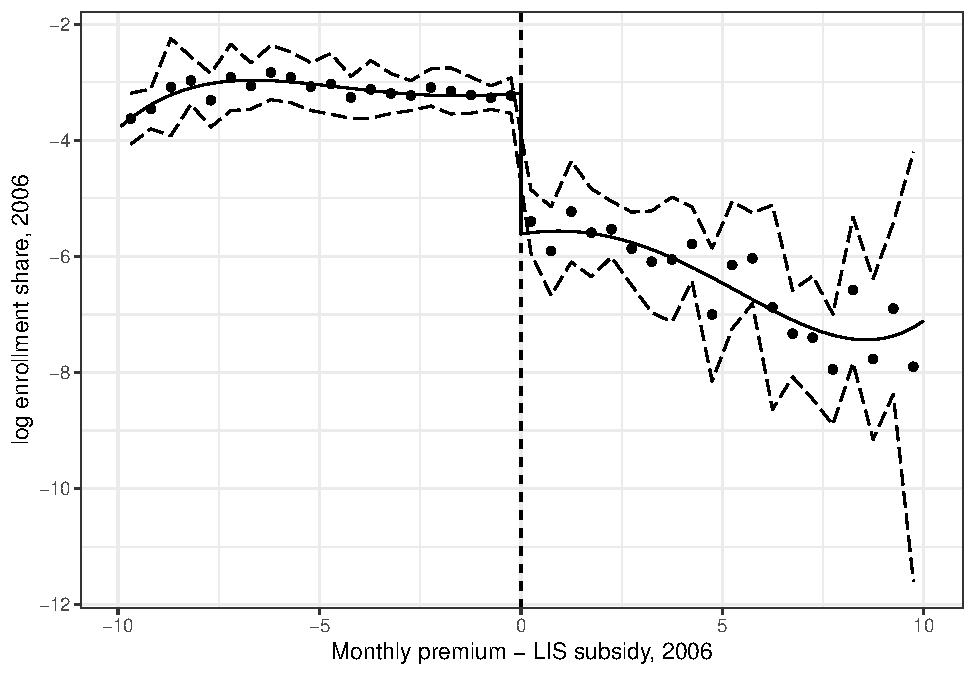
\includegraphics{solutions_files/figure-latex/rd-plot1-1.pdf}
\caption{\label{fig:rd-plot1}Intial Regression Discontinuity Plot}
\end{figure}

\newpage

\begin{figure}
\centering
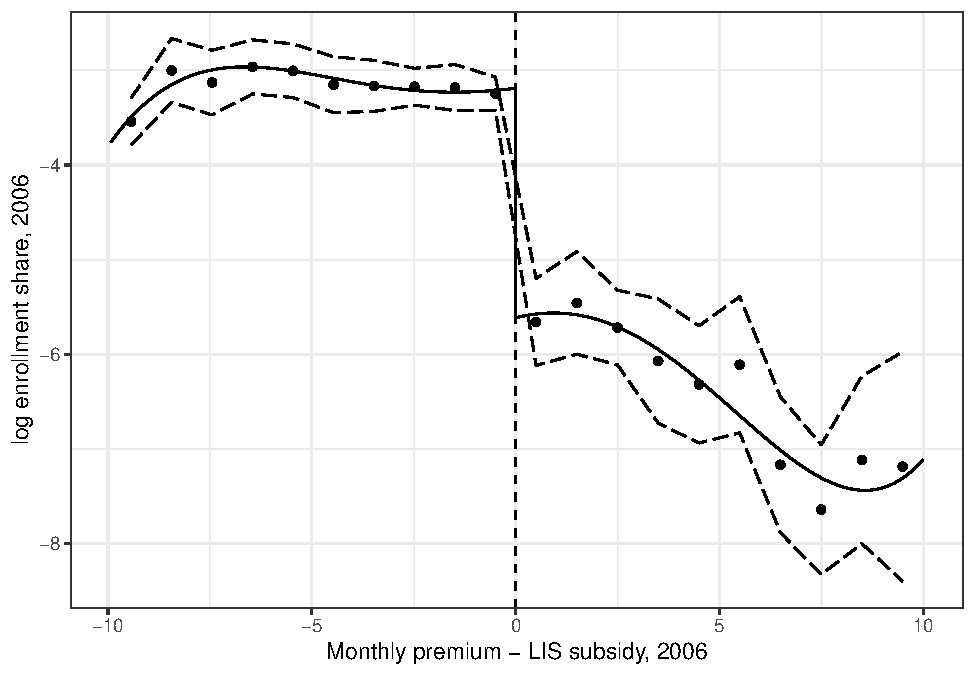
\includegraphics{solutions_files/figure-latex/rd-plot2-1.pdf}
\caption{\label{fig:rd-plot2}Regression Discontinuity Plot with Larger Bins}
\end{figure}

\newpage

\begin{figure}
\centering
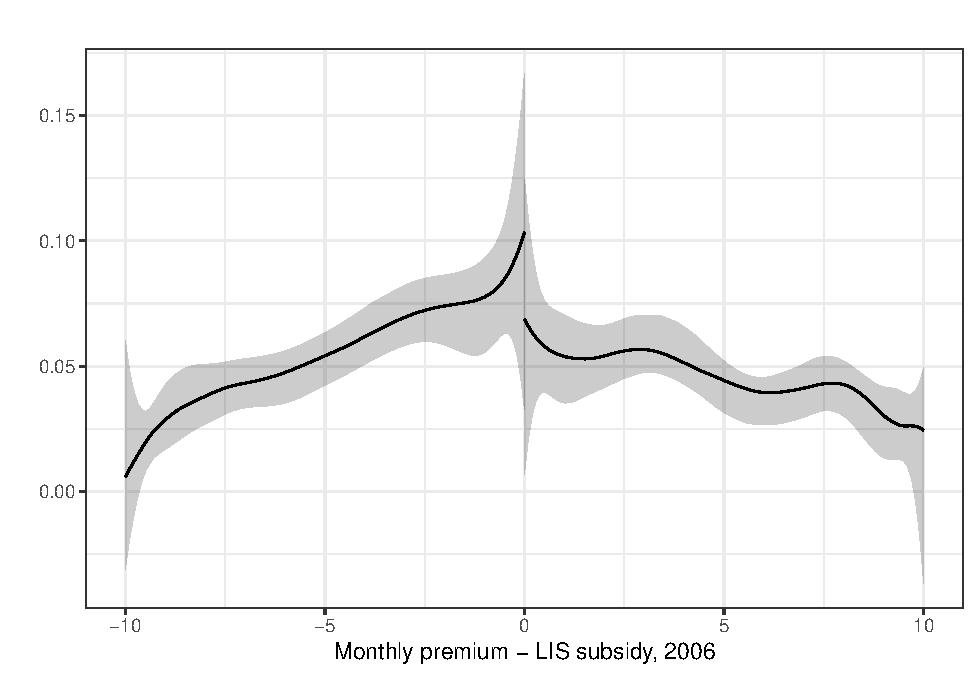
\includegraphics{solutions_files/figure-latex/rd-test-1.pdf}
\caption{\label{fig:rd-test}Test of Manipulation of Running Variable}
\end{figure}

\newpage

\begin{figure}
\centering
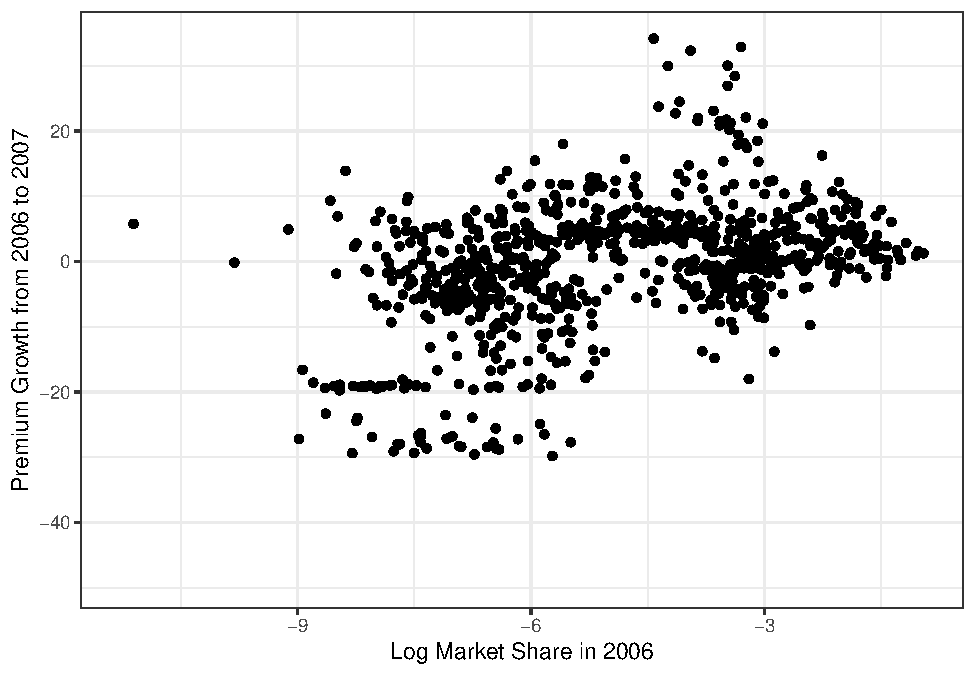
\includegraphics{solutions_files/figure-latex/scatter-1.pdf}
\caption{\label{fig:scatter}Scatterplot of Premium Changes and Market Share}
\end{figure}

\newpage

\hypertarget{references}{%
\section*{References}\label{references}}
\addcontentsline{toc}{section}{References}

\hypertarget{refs}{}
\begin{cslreferences}
\leavevmode\hypertarget{ref-ericson2014}{}%
Ericson, Keith M. 2014. ``Consumer Inertia and Firm Pricing in the Medicare Part d Prescription Drug Insurance Exchange.'' \emph{American Economic Journal: Economic Policy} 6 (1): 38--64.
\end{cslreferences}

\end{document}
